% Standalone working manuscript; numerical evidence is recorded in paper/evidence-map-001.md.
% Rewritten in place after reading the ICC papers cited as yilmaz and huang.
% IEEEtran is provisional: ICC 2027 submission requirements remain to be checked.
% Pending AP cells must be populated only from completed full-split evaluation.
\documentclass[conference]{IEEEtran}
\usepackage{amsmath,amssymb}
\usepackage{booktabs}
\usepackage{graphicx}
\usepackage{tikz}
\usetikzlibrary{arrows.meta,positioning,fit}
\usepackage{url}
\newcommand{\E}{\mathbb{E}}
\newcommand{\CN}{\mathcal{CN}}
\newcommand{\pending}{\textit{pending}}
\title{Depth-Conditioned Semantic Communication\\for Stereo 3D Object Detection}
\author{\IEEEauthorblockN{Authors to be supplied}}
\begin{document}
\maketitle
\begin{center}
\footnotesize\textit{Working draft, 5 October 2026. Full wireless detection evaluation is pending.}
\end{center}

\begin{abstract}
Wireless stereo 3D detection requires a communication representation that
retains both object appearance and depth-dependent matching information.
Reconstructing the stereo images introduces an intermediate objective whose
image-quality ranking can differ from the detection ranking. We propose a
conditional depth-field representation for transmitting stereo features to a
fixed 3D detector. At each spatial location, the encoder divides a learned
depth distribution into three equal-mass intervals and transmits their
barycenters together with conditional feature vectors. A compact appearance
code completes the packet, requiring 19 complex channel uses per location.
The receiver reconstructs the cost field at metric depth queries from the
received coordinates and features. We further formulate a receiver that
uses channel state information and node ordering to average the
reconstruction basis over a finite-grid posterior. Experiments on 3,769
KITTI stereo pairs show that higher RGB PSNR can coincide with lower 3D
average precision across source codecs. In separate simulations under a
specified ordered prior, posterior decoding reduces latent-coordinate mean
squared error from 69.3591 to 26.5377~m$^2$ over a Rayleigh channel at 10~dB.
These results characterize the motivation and receiver mechanism; the
proposed representation's end-to-end detection gain remains to be evaluated.
\end{abstract}

\begin{IEEEkeywords}
Task-oriented communication, stereo vision, 3D object detection,
joint source-channel coding, depth-conditioned features.
\end{IEEEkeywords}

\section{Introduction}
A wireless stereo perception system must convey enough visual information
for a remote detector to recognize objects and estimate their 3D locations.
These two requirements place different demands on the transmitted
representation. Appearance supports recognition, whereas left--right
correspondence determines depth. Compressing a stereo pair to improve an
image distortion measure therefore need not preserve the information most
useful to the detector. The communication problem is to allocate a limited
channel budget to the features that support the final detection decision.

Learned joint source-channel coding provides a way to optimize a transmitted
representation through a differentiable channel model. For example,
Yilmaz et al.~\cite{yilmaz} jointly encode and reconstruct images sent over a
multiple access channel. Task-oriented systems instead select features for
the intended inference task. Huang et al.~\cite{huang} use task- and
SNR-dependent feature extraction in a multi-task semantic communication
system. These designs motivate optimizing the communication interface
jointly with its reconstruction or inference objective. For stereo 3D
perception, the remaining design choice is how to represent the depth
structure on which the task depends.

Cao et al.~\cite{cao} address this problem by communicating optical-flow and
object-region information and reconstructing stereo images at the receiver.
Their image interface can be followed by an RGB-based stereo detector.
Stereo R-CNN~\cite{stereo} performs stereo object association and
region-based alignment, while LIGA-Stereo~\cite{liga} learns stereo
representations with LiDAR geometry guidance during detector training.
An alternative communication interface can be placed inside such a detector:
a sender extracts stereo features, and a receiver performs detection from
the transmitted representation. Feature communication is also studied in
collaborative perception, including digital compression and reliability-aware
feature selection in CoDS~\cite{cods}. The question here is more specific:
how should a small packet represent the joint variation of stereo features
and metric depth?

A dense bottleneck compresses the depth axis into a fixed set of latent
channels. We consider a representation whose transmitted coordinates
explicitly specify where features belong along that axis. At each pooled
spatial location, three depth barycenters summarize a learned depth
weighting, and each barycenter carries a feature conditioned on its depth
interval. The receiver uses these coordinate--feature pairs to reconstruct
the cost field required by a frozen detector. This design creates a direct
connection between the packet and its task interface: coordinate errors
move feature support along the depth axis, while feature errors change its
content. It also permits the receiver to account for uncertainty in the
received coordinates when evaluating the reconstruction basis.

This paper develops the following contributions:
\begin{itemize}
\item A conditional depth-field codec that represents each spatial location
by three equal-mass depth nodes, their associated features, and an appearance
code. The complete packet has a fixed budget of 19 complex symbols and
energy 19 per location.
\item A channel-conditioned reconstruction rule that combines the likelihood
of the received position symbols with an ordered-node prior. Finite-grid
sum-product inference provides the node marginals, which are used to
average the field basis rather than evaluate it at a single coordinate.
\item An empirical analysis of two design questions: whether RGB quality
ranks stereo detection quality consistently, and how coordinate uncertainty
affects field reconstruction. Full-split source-codec results and synthetic
channel results address these questions; matched-budget detection comparisons
are specified separately.
\end{itemize}

\section{System Model and Design Objective}
\subsection{Stereo perception interface}
We consider a calibrated stereo camera pair connected to a remote 3D
detector through a wireless link. A frozen stereo front end processes the
left and right images and produces cost features
$\mathbf c_{sd}\in\mathbb R^{32}$, appearance features
$\mathbf a_s\in\mathbb R^{32}$, and a depth guide $\pi_{sd}$.
The index $s$ denotes a spatial location and $d$ a depth query. We use
$D=72$ metric queries,
\begin{equation}
 z_d=2+\frac{57.6}{71}d\ \mathrm{m},\qquad d=0,\ldots,71.
 \label{eq:queries}
\end{equation}
These queries follow the detector's interpolation interface; the internal
cost-volume sweep has its own coordinate convention. Spatial average
pooling with stride four reduces all three tensors, and the pooled guide
is normalized across depth. The guide is a network prediction used to
weight features, rather than an assumed calibrated depth posterior.

The role of the depth axis follows from stereo geometry. For focal length
$f$, camera baseline $B$, and disparity $d_{\rm disp}$,
\begin{equation}
 Z=\frac{fB}{d_{\rm disp}},\qquad
 \Delta Z\simeq-\frac{fB}{d_{\rm disp}^{2}}\Delta d_{\rm disp}.
 \label{eq:depth}
\end{equation}
Thus a fixed disparity perturbation has a larger first-order effect at
small disparities. This motivates retaining depth-dependent feature
structure. Detection performance additionally depends on recognition and
box localization, so we optimize the codec using the detection loss.

\subsection{Wireless channel and resource constraint}
The transmitted packet $\mathbf x\in\mathbb C^N$ contains $N$ complex
channel uses and satisfies $\|\mathbf x\|_2^2=N$. For each symbol,
\begin{equation}
 y=hx+n,\qquad n\sim\CN(0,q),\qquad q=10^{-\rho/10},
 \label{eq:channel}
\end{equation}
where $\rho$ is the SNR in dB. We consider AWGN with $h=1$ and independent
Rayleigh fading with $h\sim\CN(0,1)$ for each symbol. Under perfect
receiver channel state information (CSI), zero-forcing equalization gives
$r=y/h$ with conditional noise variance $q/|h|^2$. Fades are neither
clipped nor replaced by an erasure rule. The model assumes ideal CSI and
does not include pilot or channel-estimation overhead.

Let $E_\theta$ and $R_\theta$ denote the communication encoder and decoder,
$F_0$ the frozen stereo front end, and $H_0$ the frozen detection head.
For a stereo input $\mathbf I$ with detection targets $\mathbf t$, the
training objective is
\begin{equation}
 \begin{aligned}
 \widehat{\mathbf t}
 &=H_0\bigl(R_\theta(\mathcal H(E_\theta(F_0(\mathbf I))))\bigr),\\
 \min_\theta\quad &\E\bigl[\mathcal L_{\rm det}
   (\widehat{\mathbf t},\mathbf t)\bigr],
 \end{aligned}
 \label{eq:objective}
\end{equation}
subject to the packet length and energy constraint. The expectation is over
training samples and channel realizations, and $\mathcal H$ denotes the
channel and equalization. Only the codec is optimized. The receiver knows
the shared model parameters and tensor dimensions; all sample-dependent
features and coordinates must pass through the channel.

\begin{figure*}[t]
\centering
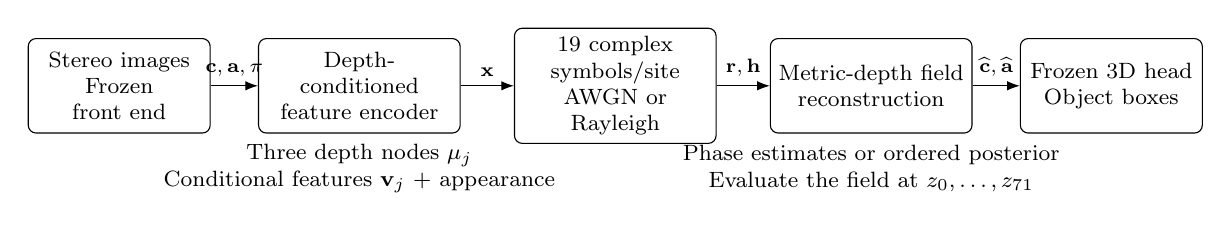
\begin{tikzpicture}[
 box/.style={draw,rounded corners=1mm,align=center,minimum height=12mm,
 text width=2.35cm,font=\footnotesize,inner sep=3pt},
 smallbox/.style={box,text width=2.1cm},
 >={Latex[length=1.6mm]}]
\node[smallbox] (front) at (0,0) {Stereo images\\Frozen front end};
\node[box] (enc) at (3.05,0) {Depth-conditioned\\feature encoder};
\node[box] (ch) at (6.3,0) {19 complex symbols/site\\AWGN or Rayleigh};
\node[box] (dec) at (9.55,0) {Metric-depth field\\reconstruction};
\node[smallbox] (head) at (12.6,0) {Frozen 3D head\\Object boxes};
\draw[->] (front)--node[above,font=\scriptsize] {$\mathbf c,\mathbf a,\pi$} (enc);
\draw[->] (enc)--node[above,font=\scriptsize] {$\mathbf x$} (ch);
\draw[->] (ch)--node[above,font=\scriptsize] {$\mathbf r,\mathbf h$} (dec);
\draw[->] (dec)--node[above,font=\scriptsize] {$\widehat{\mathbf c},\widehat{\mathbf a}$} (head);
\node[align=center,font=\footnotesize] at (3.05,-1.05)
 {Three depth nodes $\mu_j$\\Conditional features $\mathbf v_j$ + appearance};
\node[align=center,font=\footnotesize] at (9.55,-1.05)
 {Phase estimates or ordered posterior\\Evaluate the field at $z_0,\ldots,z_{71}$};
\end{tikzpicture}
\caption{Conditional depth-field communication. The encoder transmits depth
coordinates and associated features to reconstruct the detector's cost
field. Training updates the codec through the frozen detection head.
The ordered posterior is a receiver extension; the primary codec comparison
uses phase-based reconstruction.}
\label{fig:system}
\end{figure*}

\section{Conditional Depth-Field Communication}
\subsection{Depth-conditioned feature encoding}
At location $s$, a pointwise network $g_\theta$ with dimensions
$32\!\to\!16\!\to\!1$ combines the cost feature with the native depth
guide to produce normalized weights:
\begin{equation}
 p_{sd}=\operatorname{softmax}_d
 \bigl(g_\theta(\mathbf c_{sd})+\log\pi_{sd}\bigr).
 \label{eq:score}
\end{equation}
The guide is floored at the minimum positive floating-point value before
taking the logarithm. This weighting lets the codec use both the pretrained
stereo guide and the features selected by the detection objective.

To obtain a fixed-size representation, we partition the cumulative depth
mass into $K=3$ intervals. Define $F_{sd}=\sum_{t\le d}p_{st}$ and
$F_{s,-1}=0$. The mass contributed by depth atom $d$ to interval $j$ is
\begin{equation}
 m_{sjd}=\left[\min\left(F_{sd},\frac{j+1}{K}\right)
             -\max\left(F_{s,d-1},\frac{j}{K}\right)\right]_+,
 \label{eq:mass}
\end{equation}
where $j=0,1,2$ and $[v]_+=\max(v,0)$. With
$w_{sjd}=m_{sjd}/\sum_t m_{sjt}$, the transmitted node and its conditional
feature are
\begin{equation}
 \mu_{sj}=\sum_d w_{sjd}z_d,\qquad
 \mathbf v_{sj}=\sum_d w_{sjd}A_\theta(\mathbf c_{sd}),
 \label{eq:barycenters}
\end{equation}
where $A_\theta:\mathbb R^{32}\to\mathbb R^8$ is a learned pointwise
map. Each node summarizes one third of the depth mass in exact arithmetic,
and the interval construction orders the barycenters. It retains three
conditional summaries rather than collapsing all depth support into one
mean. This is a representation choice; its suitability for detection is
tested against a dense depth bottleneck in Section~\ref{sec:evaluation}.
% Numerical validation of ordering for every stored float32 packet remains pending.

\subsection{Channel mapping and field reconstruction}
We encode each barycenter as a unit-energy phase symbol,
\begin{equation}
 x_{sj}=e^{i\vartheta_{sj}},\qquad
 \vartheta_{sj}=\pi\frac{\mu_{sj}-2}{57.6}-\frac{\pi}{2}.
 \label{eq:phase}
\end{equation}
Each eight-dimensional real feature is paired into four complex symbols
and normalized jointly to energy four. A separate
$32\!\to\!8$ appearance encoder produces another four-symbol group
with energy four. The packet therefore contains
\begin{equation}
 N= N_{\rm sites}\underbrace{(3+3\cdot4+4)}_{\text{positions + features + appearance}}
   =19N_{\rm sites}
 \label{eq:budget}
\end{equation}
complex symbols, with the same total energy. The fixed detector interface
has 1,560 pooled locations, giving 29,640 complex uses per stereo frame.
Normalization retains feature direction; discarded magnitudes are not sent
as side information. Near-zero feature groups use a fixed sphere point.

For the primary receiver, the equalized position symbols are projected
onto the unit circle. Their phases are clipped to $[-\pi/2,\pi/2]$ and
mapped back to coordinates $\widehat\mu_{sj}\in[2,59.6]$~m.
Each received feature group is projected onto its known energy-four sphere
and decoded with $D_\theta:\mathbb R^8\to\mathbb R^{32}$. The reconstructed
cost field is
\begin{equation}
 \widehat{\mathbf c}_{sd}=\frac{1}{3}\sum_{j=0}^{2}
 \exp\!\left[-\frac{(z_d-\widehat\mu_{sj})^2}{2\sigma^2}\right]
 D_\theta(\widehat{\mathbf v}_{sj}),
 \label{eq:field}
\end{equation}
where $\sigma>0$ is a learned scalar shared across all locations. The
Gaussian basis places each decoded feature around its received depth
coordinate. Its weights are not normalized across nodes. An independent
$8\!\to\!32$ map decodes appearance. Trilinear interpolation restores the
cost tensor and bilinear interpolation restores the appearance tensor to
the shapes consumed by the frozen detection head.

\subsection{Reconstruction under coordinate uncertainty}
A point estimate in~\eqref{eq:field} treats an uncertain position symbol
as one known coordinate. Under fading, equalized observations can have
very different reliabilities. We therefore consider a receiver extension
that averages the basis using the coordinate likelihood and node ordering.
This extension changes neither the transmitted packet nor its energy.

Suppress the spatial index and write $u_j=(\mu_j-2)/57.6$. On a shared
grid $\{u_m\}_{m=1}^M\subset[0,1]$, the position log-likelihood,
up to terms independent of $m$, is
\begin{equation}
 \ell_j(m)=\frac{2|h_j|^2}{q}
 \Re\!\left\{r_j e^{-i\pi(u_m-1/2)}\right\}.
 \label{eq:likelihood}
\end{equation}
The factor $|h_j|^2/q$ accounts for the actual reliability of the equalized
observation. We use a uniform prior over ordered grid triples
$a\le b\le c$, including ties. For $L_j(m)=e^{\ell_j(m)}$, the forward
messages are
\begin{align}
 A_1(m)&=L_1(m),\nonumber\\
 A_2(m)&=L_2(m)\sum_{t\le m}A_1(t),\nonumber\\
 A_3(m)&=L_3(m)\sum_{t\le m}A_2(t).
 \label{eq:forward}
\end{align}
The backward messages satisfy $B_3(m)=1$,
$B_2(m)=\sum_{t\ge m}L_3(t)$, and
$B_1(m)=\sum_{t\ge m}L_2(t)B_2(t)$. The marginal for node $j$ is
$A_j(m)B_j(m)/\sum_t A_3(t)$. Log-domain prefix and suffix sums compute
these marginals in $O(3M)$ operations using standard sum-product inference.

The posterior-averaged basis weight is
\begin{equation}
 \overline k_{jd}=\frac{1}{3}\sum_m p(u_j=u_m\mid\mathbf r,\mathbf h)
 \exp\!\left[-\frac{(z_d-2-57.6u_m)^2}{2\sigma^2}\right].
 \label{eq:expectedbasis}
\end{equation}
The receiver substitutes these weights into~\eqref{eq:field} while keeping
the feature and appearance decoders fixed. Because the basis is nonlinear,
evaluating it at the posterior-mean coordinate generally differs from
averaging its values. The latter estimates the basis under the assumed
posterior and is the quantity examined in the synthetic field experiment.
The model omits feature--coordinate dependencies, and its uniform ordered
prior is not fitted to the learned KITTI coordinates. We use 289 grid
points for receiver integration; the synthetic validation in
Section~\ref{sec:synthetic} uses a separate 33-point source prior.

\subsection{Task-driven codec training}
We optimize the codec with the detector's native classification and
box-regression loss, including localization, IoU, and direction terms.
The stereo front end and detection head remain frozen throughout training.
LIGA-Stereo's original pretraining uses LiDAR guidance~\cite{liga}; codec
training uses stereo images and detection labels without an additional
RGB reconstruction or depth-supervision loss.

Each codec is trained on 3,712 stereo pairs for three epochs using Adam,
learning rate $10^{-3}$, and zero weight decay. Training samples AWGN and
Rayleigh channels with equal probability and draws SNR continuously from
$[6,18]$~dB. Seed 17 fixes the frame order and channel schedule. Compared
codecs use paired noise and fading realizations. This setup optimizes the
communication representation for the same fixed task receiver and channel
range.

\section{Experimental Results}
\label{sec:evaluation}
\subsection{Evaluation setup and comparisons}
Evaluation uses all 3,769 pairs of the fixed KITTI validation split. The
detection metric is Car 3D Moderate AP$_{R40}$ at IoU 0.7. The primary
comparison uses the third-epoch checkpoint at AWGN 10~dB, without selecting
checkpoints by validation AP. The planned channel sweep covers AWGN at
integer SNRs from 6 to 18~dB and Rayleigh at 6, 8, 10, 12, 14, 16, and
18~dB, together with an identity-channel reference.

Table~\ref{tab:arms} defines the four codecs. P denotes the proposed
guide-conditioned field codec. G removes the guide term from
\eqref{eq:score}, while S circularly shifts the guide by half the pooled
height and width. These controls test guide usage and its spatial
correspondence. B is a dense codec that concatenates the centered log guide
with the cost features, applies a $33\!\to\!10$ feature map and learned
$72\!\to\!3\!\to\!72$ depth maps, and reconstructs the cost channels
with a $10\!\to\!32$ map. Its 15 complex feature symbols form one
energy-15 group; the appearance interface is shared with the field codecs.

\begin{table}[t]
\centering
\caption{Codec comparisons at a common budget of 19 complex symbols and
energy 19 per spatial location. Parameter counts exclude the frozen detector.}
\label{tab:arms}
\begin{tabular}{llllr}
\toprule
Codec & Representation & Guide & Positions & Params.\\
\midrule
G & Conditional field & None & 3 & 1,650\\
P & Conditional field & Aligned & 3 & 1,650\\
S & Conditional field & Shifted & 3 & 1,650\\
B & Dense bottleneck & Aligned & 0 & 1,751\\
\bottomrule
\end{tabular}
\end{table}

P--B compares complete architectures with the same channel budget, including
their different parameter counts and feature normalization groups. P--G and
P--S isolate changes within the field architecture. The primary comparison
uses phase-based decoding; the posterior extension is evaluated separately.
Full-split learned-codec AP is pending in Table~\ref{tab:pending}. The
completed results below concern source compression and synthetic receiver
estimation. The single training seed does not quantify training variability.

\begin{table}[t]
\centering
\caption{End-to-end detection comparison to be completed. Third-epoch
checkpoints; 3,769 validation pairs; AWGN 10~dB; Car 3D Moderate
AP$_{R40}$ at IoU 0.7.}
\label{tab:pending}
\begin{tabular}{lrrrr}
\toprule
Codec & G & P & S & B\\
\midrule
AP (\%) & \pending & \pending & \pending & \pending\\
\bottomrule
\end{tabular}
\end{table}

\subsection{Image quality and detection quality}
We first examine whether image quality consistently ranks stereo detection
performance. JPEG and JPEG2000 reconstructions at nominal compression
ratios (CRs) of 10, 30, and 50 are evaluated with frozen Stereo R-CNN and
LIGA-Stereo detectors. These experiments cover the full validation split
and contain no wireless channel. Actual CR is the total raw RGB byte count
divided by the total compressed byte count. PSNR is calculated from pooled
full-image RGB MSE.

\begin{table*}[t]
\centering
\caption{Source-compression results on 3,769 KITTI stereo pairs without
channel noise. AP is Car 3D Moderate AP$_{R40}$ at IoU 0.7 (\%). Actual
source rates differ at each nominal setting, as reported by CR and mean
bytes per stereo pair.}
\label{tab:rgb}
\begin{tabular}{lrrrrrr}
\toprule
Source codec & Nominal CR & Actual CR & Bytes/pair & PSNR (dB) & Stereo R-CNN AP & LIGA AP\\
\midrule
JPEG & 10 & 11.019 & 252,943 & 29.915 & 33.883 & 65.019\\
JPEG2000 & 10 & 10.004 & 278,596 & 36.093 & 32.188 & 62.650\\
JPEG & 30 & 33.205 & 83,937 & 27.993 & 29.947 & 56.954\\
JPEG2000 & 30 & 30.018 & 92,849 & 30.438 & 28.557 & 51.681\\
JPEG & 50 & 54.666 & 50,985 & 26.803 & 20.797 & 44.571\\
JPEG2000 & 50 & 50.037 & 55,702 & 28.652 & 25.228 & 45.458\\
\bottomrule
\end{tabular}
\end{table*}

Table~\ref{tab:rgb} shows a ranking discrepancy at nominal CRs 10 and 30.
At CR 10, JPEG2000 yields 36.093~dB PSNR, compared with 29.915~dB for JPEG,
yet its LIGA AP is 62.650\%, compared with 65.019\% for JPEG. Stereo R-CNN
exhibits the same direction of change. At CR 50, JPEG2000 improves both
PSNR and AP. Thus PSNR does not consistently order downstream detection
quality across these operating points. This observation motivates a task
loss and a representation tied to the detector's depth features. The
unequal source rates and different codec artifacts do not identify the
cause of the discrepancy or establish a matched-rate advantage.

\subsection{Coordinate and field reconstruction over the channel}
\label{sec:synthetic}
To examine the receiver independently of detector training, we sample
65,536 triples per channel condition from a uniform prior over all 6,545
inclusive ordered triples on a 33-point grid. Each triple is transmitted
using three unit-energy position symbols. The 20 AWGN and Rayleigh
conditions use the SNR grids specified above, giving 1,310,720 trials.
The source prior matches the posterior model in this experiment.

\begin{table}[t]
\centering
\caption{Synthetic coordinate MSE at 10~dB under the ordered 33-point
prior. Values are scaled by $57.6^2$ into m$^2$ and describe transmitted
latent coordinates, not detected object depths.}
\label{tab:receiver}
\begin{tabular}{lrr}
\toprule
Receiver & AWGN & Rayleigh\\
\midrule
Clipped phase & 16.1234 & 69.3591\\
Independent uniform-slot posterior & 15.4297 & 46.4875\\
Weighted isotonic projection & 14.3532 & 40.8337\\
Ordered fading-blind posterior & 12.9310 & 31.5355\\
Ordered CSI-conditioned posterior & 12.9310 & 26.5377\\
\bottomrule
\end{tabular}
\end{table}

Table~\ref{tab:receiver} reports the coordinate errors at 10~dB. Under
Rayleigh fading, conditioning on the actual CSI reduces MSE from 31.5355
for the fading-blind ordered receiver to 26.5377. The two receivers coincide
under AWGN, where all symbols have the same channel gain. This comparison
illustrates the value of weighting coordinate observations by their
conditional reliability. The independent uniform-slot posterior has
different marginal priors from the ordered model, so its comparison with
the ordered receiver combines marginal-prior and inter-node effects.
Isolating the ordering effect requires a matched-marginal control.

We also reconstruct a scalar field using fixed coefficients
$(0.8,-0.3,0.5)$, nine query locations, and bandwidth $1/3$ in normalized
coordinates. Posterior basis averaging gives field MSEs of 0.00059813
under AWGN and 0.00110864 under Rayleigh. Substituting posterior-mean
coordinates into the basis gives 0.00060495 and 0.00116890, respectively.
These results are consistent with estimating the nonlinear basis directly
under the specified posterior. They quantify a receiver mechanism under
its assumed source model; transferring this gain to trained stereo
features requires end-to-end detection evaluation.

\subsection{Scope of the current evidence}
The proposed interface requires the sender to compute stereo cost features
and the receiver to use the corresponding detection head. Its small codec
parameter count therefore does not measure total sender complexity. The
current model also uses a fixed symbol budget, a global basis bandwidth,
and perfect CSI. The posterior extension introduces a grid prior and
additional computation whose effect on detector accuracy and latency
remains unmeasured.

A complete wireless comparison must express digital baselines in channel
uses after quantization, framing, channel coding, modulation, and required
side information. Source byte ratios alone cannot be compared with the
analog budget in~\eqref{eq:budget}. Flow/ROI, SRCNN, and KITTI-adapted ECSIC
baselines, full detection curves, and sender/receiver resource measurements
remain to be completed. The available evidence supports the image/task
ranking observation and the synthetic receiver analysis, while leaving
the central matched-budget detection comparison open.

\section{Conclusion}
We proposed a semantic communication interface that represents a stereo
cost field through depth coordinates and conditional features. Equal-mass
depth summaries give a fixed 19-symbol packet per location, and the
receiver reconstructs the field at the detector's metric queries. An
ordered posterior extends this reconstruction to account for channel-dependent
coordinate uncertainty. Completed experiments reveal an RGB-quality/detection
ranking discrepancy and lower synthetic estimation error under the stated
prior. Full-split wireless detection and resource comparisons are needed
to determine whether the representation improves the accuracy--communication
tradeoff for stereo 3D perception.

\begin{thebibliography}{00}
\bibitem{yilmaz}
S. F. Yilmaz, C. Karamanli, and D. G\"und\"uz,
``Distributed Deep Joint Source-Channel Coding over a Multiple Access Channel,''
in \emph{Proc. IEEE International Conference on Communications (ICC)}, 2023.
\bibitem{huang}
S.-Y. Huang, R. Liao, and V. W. S. Wong,
``Leveraging MoE-Based Large Language Model for Zero-Shot Multi-Task Semantic
Communication,'' in \emph{Proc. IEEE International Conference on
Communications (ICC)}, 2025.
\bibitem{cao}
Z. Cao, H. Zhang, L. Liang, H. Wang, S. Jin, and G. Ye Li,
``Task-Oriented Semantic Communication for Stereo-Vision 3D Object Detection,''
\emph{IEEE Transactions on Communications}, vol. 73, no. 9,
pp. 7552--7567, 2025, doi: 10.1109/TCOMM.2025.3545687.
\bibitem{stereo}
P. Li, X. Chen, and S. Shen,
``Stereo R-CNN Based 3D Object Detection for Autonomous Driving,''
in \emph{Proc. IEEE/CVF CVPR}, 2019, pp. 7644--7652.
\bibitem{liga}
X. Guo, S. Shi, X. Wang, and H. Li,
``LIGA-Stereo: Learning LiDAR Geometry Aware Representations for Stereo-Based
3D Detector,'' in \emph{Proc. IEEE/CVF ICCV}, 2021, pp. 3153--3163.
\bibitem{cods}
J. Gan, L. Liang, H. Zhang, C. Guo, and S. Jin,
``CoDS: Collaborative Perception via Digital Semantic Communication,''
\emph{arXiv:2512.22513v1}, 2025.
\end{thebibliography}
\end{document}
